\section{系统设计与方法}

\subsection{系统全貌与职责划分}
Cloudra 根据规定的反应条件与计算要求，通过构造候选分子构型、寻找和表征驻点、追踪基元反应路径及比较竞争通道研究反应机理。工作流图按照执行依赖组织工具调用与计算任务。Cloudra 的 Delivery DAG 表达所交付的反应机理：节点是物种在反应序列中的一次出现，边是基元反应步骤。智能体须在该化学图中表达候选物种及其反应连接，再根据机理假设和返回的计算结果选择后续几何操作、计算与探索分支。

规范拓扑和立体构型比较用于判断结构所表示的物种，原子映射确定反应物与产物构型中哪些原子相互对应。几何算子旋转、平移和组装分子片段。频率计算判断驻点曲率；IRC 及其后的端点优化和频率分析确定鞍点连接哪些物种。

协调智能体提出机理假设和候选基元反应步，并选择要探索的分支。计算智能体调用几何算子构造三维结构，提交所分配反应步的量子化学计算。若出现几何发散、鞍点优化收敛失败或路径分叉，计算智能体检查结构和计算诊断，判断是否继续该步骤。若认为该步骤受阻，则向协调智能体说明诊断结果，由其修改假设或探索另一分支。督导智能体对照任务要求审阅 DAG 中的物种、反应步和计算结果；审阅意见与计算输出中解析出的事实分别保存。

\begin{figure*}[!tbp]
\centering
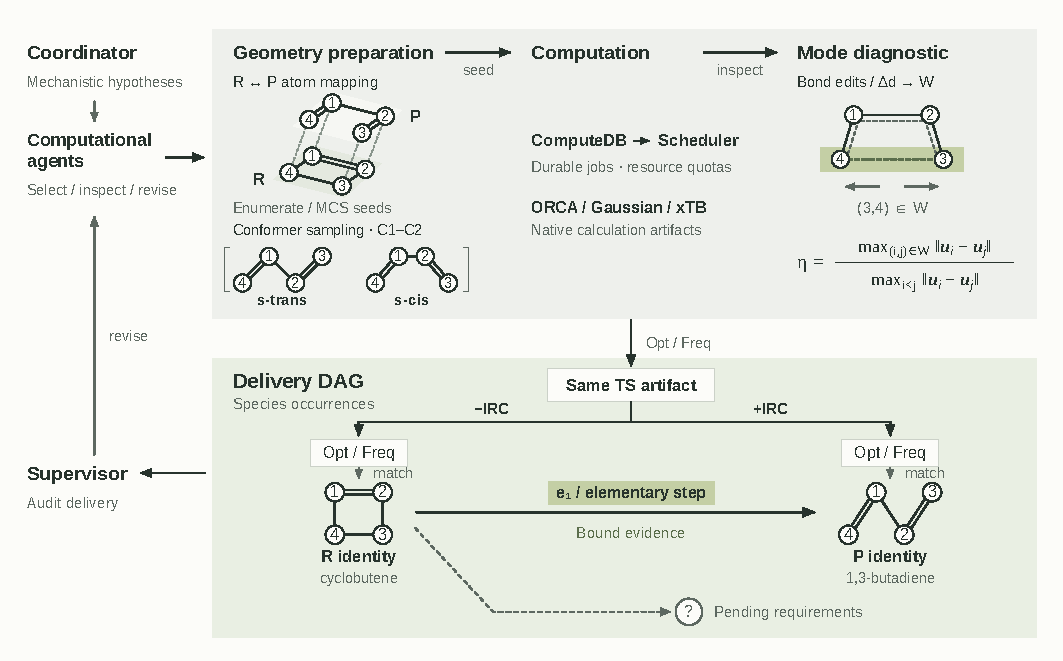
\includegraphics[width=\textwidth]{figures/Cloudra_Architecture_Stacked.pdf}
\caption{Cloudra 的机理探索流程。原子映射与构象采样用于准备反应物和产物结构，ComputeDB 与调度器管理计算。振动模式诊断测量监控原子对的运动。双向 IRC 从同一过渡态出发，两侧外帧分别用于端点优化和频率分析，再将所得结构与交付 DAG 中声明的物种比较。督导智能体审阅该图，列出待完成的计算和待确定的结构与路径归属。}
\label{fig:04}
\end{figure*}

\subsubsection{异步计算调度与资源管理}
计算数据库（\texttt{ComputeDB}）记录每个作业的状态。独立容量池分别限制本地工作进程、远程 SSH 集群和 Slurm 队列中的并发计算数。提交前，调度器根据 Cartesian 坐标、自旋、电荷及理论级别计算 SHA-256 摘要；若有相同的在运行作业或缓存结果，则直接复用，避免重复提交。操作系统的文件排他锁（\texttt{flock}）用于跟踪运行进程和并发数；监控异常期间，持有锁的量子化学进程继续运行。计算结束后，调度器通知计算智能体，由通知触发异步读取输出。

\subsection{分子表征与几何算子}
分子输入包括属性图 $H=(A,B)$ 和 Cartesian 坐标矩阵 $\mathbf{X}\in\mathbb{R}^{n\times 3}$。其中 $A$ 为原子集合，$B$ 为化学键集合，$\mathbf{X}$ 的每一行给出一个原子的坐标。图中记录原子与化学键属性。几何算子修改坐标并返回所得结构的测量值；替换原子或官能团时也修改 $H$。

\subsubsection{原子对应关系与反应中心感知}
原子属性显式保留元素种类、同位素标号、形式电荷、显式氢数、自由基电子数以及声明的手性立体构型；化学键属性保留键级与顺反立体构型。已有坐标予以保留，其余分子组分由 ETKDGv3 算法生成初始三维构象 \citep{ref12,etkdg2020,ref13}，多组分体系分别构建后执行空间对接。两端均具有完整且唯一的原子映射标号时，直接依据标号配对原子，要求两端元素与同位素相同。其余情况下，设产物与反应物的重原子集合分别为 $A_{\mathrm{P}}$ 与 $A_{\mathrm{R}}$，搜索保持元素与同位素守恒的双射 $\pi:A_{\mathrm{P}}\to A_{\mathrm{R}}$，满足 $z_i^{\mathrm{P}}=z_{\pi(i)}^{\mathrm{R}}$ 且 $\iota_i^{\mathrm{P}}=\iota_{\pi(i)}^{\mathrm{R}}$，并按下式打分：

\begin{equation}\label{eq:methods-01}
\begin{aligned}
J(\pi)={}&2(N_{\mathrm{f}}+N_{\mathrm{b}})+N_{\mathrm{o}}\\
&+4\Delta_H+8\Delta_q+8\Delta_r+2N_{\mathrm{s}}.
\end{aligned}
\end{equation}

令 $B_{\mathrm{P}}^\pi$ 表示以反应物原子编号表示的产物化学键集合。成键与断键分别是集合差 $B_{\mathrm{P}}^\pi\setminus B_{\mathrm{R}}$ 与 $B_{\mathrm{R}}\setminus B_{\mathrm{P}}^\pi$，对应基数分别为 $N_{\mathrm{f}}$ 与 $N_{\mathrm{b}}$。$N_{\mathrm{o}}$ 统计 $B_{\mathrm{P}}^\pi\cap B_{\mathrm{R}}$ 中键级改变的键对数。对于 $a\in\{H,q,r\}$，环境差量定义为 $\Delta_a=\sum_{i\in A_{\mathrm{P}}}|a_i^{\mathrm{P}}-a_{\pi(i)}^{\mathrm{R}}|$，分别度量原子显式氢数、形式电荷与未配对电子数的变化。$N_{\mathrm{s}}$ 统计立体化学环境的差异数：仅一端声明四面体标签时增加惩罚 2；当两端对应原子均声明立体标签时，算法要求其具备四个匹配邻居（含必要氢原子），并在比较标签前校正邻居排序的置换奇偶性；两端标签的差异仅在四个邻居可匹配时计分。

对于各元素同位素等价类（大小记为 $n_g$），全排列空间大小为 $N_\Pi=\prod_g n_g!$。当 $N_\Pi\le 10^5$ 时，算法遍历全部双射；超过该阈值时，以最大公共子图（MCS）作为种子扩展映射，要求元素严格匹配、放开键级限制并强制保留完整环结构 \citep{ref13}。MCS 搜索超时时间为 10 秒，每个端点最多贡献 64 个子图匹配。剩余原子按氢数、连接度及输入序号在同类原子中排序配对。算法合并成断键、键级变化及得分相同的映射，保留字典序最小的代表；候选按得分与映射序列升序排序，前 16 个代表构成重原子候选集 $C$。当 $C$ 包含候选映射时，定义最优得分 $J_{\min}=\min_{\pi\in C}J(\pi)$ 以及容差集合 $\mathcal{N}=\{\pi\in C:J(\pi)\le J_{\min}+2\}$。当 $|\mathcal{N}|=1$ 时报告映射唯一；$|\mathcal{N}|>1$ 时报告存在歧义；$C=\emptyset$ 时将映射结果标记为待定。

每个保留的重原子候选映射按与两端图相容的原子匹配扩展至全原子。系统优先保留相容的显式氢标号，再按同位素配对各对应重原子上的剩余氢原子。剩余氢原子组（大小为 $h_g$）的置换空间 $N_H=\prod_g h_g!$ 在 $N_H<257$ 时执行完全枚举；超出该范围时，需要相容的显式氢标签来确定配对；仍有配对歧义时，将结果标记为待定。全原子映射经过去重、排序，并依据相同的 $+2$ 容差规则评估歧义性。选定的全原子双射将产物原子排成反应物的原子顺序。成键与断键原子对用于监控后续路径插值；键级变化随变换后的拓扑图一同记录。

\subsubsection{结构测量与刚体变换算子}
系统根据坐标计算键长、键角、二面角、环构象和近距离接触。对于坐标 $\mathbf{x}_i$，原子间距为 $d_{ij}=\|\mathbf{x}_j-\mathbf{x}_i\|$；以原子 $j$ 为顶点的键角由两条成键单位向量的内积反余弦求得。将原子间距与参考键长和范德华接触距离比较，标记几何异常。纯坐标输入在进入系统时确定成键拓扑；局部坐标变换保留该键图，并在移动原子前后重复测量。

对于非环单键两侧的分子片段选择，系统通过图连通性自动解析：临时切断指定键 $a-b$，选取包含原子 $b$ 的连通子图 $\mathcal{F}_b$。若切除该键后两端依然连通（处于环体系内部），则要求显式传入移动原子列表。记移动原子集合为 $\mathcal{F}$（由显式指定或切键提取的 $\mathcal{F}_b$ 构成）。将移动片段绕指定空间轴旋转时，对集合内所有原子 $i\in\mathcal{F}$ 应用 Rodrigues 旋转公式：

\begin{equation}\label{eq:methods-02}
\begin{aligned}
\mathbf{x}_i'&=\mathbf{a}+\mathbf{R}(\hat{\mathbf{u}},\theta)(\mathbf{x}_i-\mathbf{a}),\\
\mathbf{R}&=\cos\theta\,\mathbf{I}+(1-\cos\theta)\hat{\mathbf{u}}\hat{\mathbf{u}}^{\mathsf{T}}\\
&\quad+\sin\theta\,[\hat{\mathbf{u}}]_\times.
\end{aligned}
\end{equation}

式中 $\mathbf{a}$ 为旋转轴上基准点，$\hat{\mathbf{u}}$ 为轴的单位方向向量，$\theta$ 为旋转角度，$\mathbf{I}$ 为三阶单位矩阵，$[\hat{\mathbf{u}}]_\times\mathbf{v}=\hat{\mathbf{u}}\times\mathbf{v}$ 为反对称叉乘算子。移动片段之外的原子坐标固定。沿指定键 $a-b$ 伸缩距离时，将片段 $\mathcal{F}_b$ 整体平移：

\begin{equation}\label{eq:methods-03}
\mathbf{x}_i'=\mathbf{x}_i+(L-d_{ab})\frac{\mathbf{x}_b-\mathbf{x}_a}{d_{ab}},\qquad i\in\mathcal{F}_b.
\end{equation}

式中 $L$ 为目标键长，$\mathcal{F}_b$ 之外的原子坐标固定。手性反转通过绕立体中心旋转两个可分离分支，交换两个分支的方向。基团取代先移除指定侧片段，再沿原连接键的方向放置新基团，并更新拓扑图。比较量子化学优化前后的结构时，系统保持相同元素顺序，分别按距离判断成键，再比较新增或消失的连接属于片段内部还是片段之间。

\subsubsection{分支拥挤描述符与反应物预组织}
检查杂化状态、环结构和取代基拓扑不等价性后，系统根据各取代基分支中的原子计算候选旋转轴周围的拥挤程度：

\begin{equation}\label{eq:methods-04}
B_s=\sum_{k\in T_s} c_k r_k \rho^{\ell_k},\qquad\rho=0.5,\quad 0\le \ell_k\le 5.
\end{equation}

式中 $r_k$ 为原子 $k$ 的范德华半径。遍历树 $T_s$ 通过后进先出（LIFO）深度优先遍历生成，以取代基根原子为深度 0 起点，并将旋转轴另一端原子预先标记为已访问。弹出待访问原子时记录其搜索深度 $\ell_k$，并在 $\ell_k<5$ 时将其待访问邻居按拓扑顺序压栈。权重系数 $c_k$ 在根原子图连接度大于等于 3 时取 1.5，其余原子取 1.0。

该描述符采用标准范德华半径标度（Å）：H 1.20, B 1.92, C 1.70, N 1.55, O 1.52, F 1.47, P 1.80, S 1.80, Cl 1.75, Br 1.85, I 1.98（其余元素统一采用 1.70）。将旋转轴两侧四个取代基分支计算得出的 $B_s$ 值四舍五入保留三位小数并求和，其总和记为 $B_{\mathrm{axis}}$；当 $B_{\mathrm{axis}}\ge 9.0$ 时，该键被标记为拥挤轴，供后续构象探查参考。

在多组分反应物预组织中，主反应组分固定于坐标原点，其余反应物分子绕各自质心在三维空间中进行取向采样。在 $K$ 个采样点下，第 $s$ 个采样方向为：

\begin{equation}\label{eq:methods-05}
\begin{aligned}
\hat{\mathbf{u}}_s&=(a_s\cos s\gamma,\,y_s,\,a_s\sin s\gamma),\\
a_s&=\sqrt{1-y_s^2},\qquad y_s=1-\frac{2s}{K-1},\\
\gamma&=\pi(3-\sqrt{5}).
\end{aligned}
\end{equation}

其中参数 $\gamma=\pi(3-\sqrt{5})\approx 2.3999\text{ rad}$（约为 $137.5^\circ$）为黄金角，对应斐波那契球面螺旋分布；绕 $\hat{\mathbf{u}}_s$ 轴的自旋角取 $2\pi s/K$（默认采样 $K=32$）。沿组分质心向量平移以消除原子重叠冲突。对于显式指定的引导原子对集合 $W$ 及其目标距离窗口 $[l_{ij},u_{ij}]$，构型 $\mathbf{X}$ 的违背惩罚评分为：

\begin{equation}\label{eq:methods-06}
\begin{aligned}
S(\mathbf{X})=\max_{(i,j)\in W}\{&0,\,l_{ij}-d_{ij}(\mathbf{X}),\\
&d_{ij}(\mathbf{X})-u_{ij}\}.
\end{aligned}
\end{equation}

低惩罚构型进行带谐性距离约束的 MMFF94 力场优化\citep{mmff941996}，使指定原子对的距离进入目标窗口，同时松弛非键接触。只保留力场优化收敛、距离落入窗口、立体构型得到保留且片段接触满足 $d_{i^*j^*}\le 1.7(r_{i^*}+r_{j^*})$ 的构型。随后按无约束力场单点能排序，并采用 0.5 Å 的重原子 Kabsch RMSD 阈值聚类去重，得到后续计算的初始构型。

\subsubsection{端点刚体对齐与 IDPP 路径插值}
将产物原子排成反应物的原子顺序后，两端构型分别中心化。令 $\mathbf{P}$ 与 $\mathbf{R}$ 为中心化后的产物与反应物坐标矩阵，Kabsch 最小二乘刚体旋转\citep{ref07}\ 求解：

\begin{equation}\label{eq:methods-07}
\begin{gathered}
\min_{\mathbf{Q}^{\mathsf{T}}\mathbf{Q}=\mathbf{I},\det\mathbf{Q}=1}\|\mathbf{P}\mathbf{Q}-\mathbf{R}\|_{\mathrm{F}}^2,\\
\mathbf{P}^{\mathsf{T}}\mathbf{R}=\mathbf{U}\boldsymbol{\Sigma}\mathbf{V}^{\mathsf{T}},\\
\mathbf{Q}=\mathbf{U}\operatorname{diag}\!\bigl(1,1,\det(\mathbf{U}\mathbf{V}^{\mathsf{T}})\bigr)\mathbf{V}^{\mathsf{T}}.
\end{gathered}
\end{equation}

矩阵 $\mathbf{Q}$ 给出两端构型之间的刚体旋转。行列式因子 $\det(\mathbf{U}\mathbf{V}^{\mathsf{T}})$ 使 $\det\mathbf{Q}=+1$，排除镜像反射，保留原有手性构型。

对于包含端点在内的 $M$ 个路径帧，定义进度参数 $\lambda_k=k/(M-1)$，并初始化坐标 $\mathbf{X}_k=(1-\lambda_k)\mathbf{R}+\lambda_k\mathbf{P}\mathbf{Q}$。IDPP 算法\citep{ref08}\ 在两端之间插值各帧的目标原子对距离，并按下式优化坐标：

\begin{equation}\label{eq:methods-08}
\begin{aligned}
d_{ij,k}^*&=(1-\lambda_k)d_{ij}^{\mathrm{R}}+\lambda_k d_{ij}^{\mathrm{P}},\\
V_k&=\sum_{i<j}\frac{(d_{ij,k}-d_{ij,k}^*)^2}{d_{ij,k}^4}.
\end{aligned}
\end{equation}

该泛函的分母引入距离负四次方权重 $d_{ij,k}^{-4}$，使短程成键区域具有较高的刚性恢复力，优先保持化学键尺度，同时允许长程非键相互作用松弛。标准模式将中间镜像帧通过改进切线法弹性带（NEB）弹簧耦合，并利用 MDMin 算法执行能量最小化，以移动原子受力的最大残差评估收敛性\citep{neb2000,ase2017}；轻量模式则将分母设定为 $\max(d_{ij,k}^*,0.1\,\text{Å})^4$，使用 Adam 优化器对各个中间镜像帧独立进行几何松弛。\citep{adam2015}

动态监控原子对集合 $W$ 自动提取反应映射中的成断键对、两端成键但键长变化 $|\Delta d|\ge 0.15$ Å 的键对，以及两端距离变化最大的前 5 对原子。在集合 $W$ 中，主反应坐标及其中点距离为：
\[
\begin{aligned}
p^*&\in\operatorname{argmax}_{p\in W}|d_p^{\mathrm{P}}-d_p^{\mathrm{R}}|,\\
m&=(d_{p^*}^{\mathrm{R}}+d_{p^*}^{\mathrm{P}})/2.
\end{aligned}
\]
初始过渡态初猜选取首个跨越中点的镜像帧 $k$（满足 $(d_{p^*,k}-m)(d_{p^*}^{\mathrm{R}}-m)\le 0$），或与中点距离偏差最小的帧。提取出的三维构型直接作为后续一阶鞍点优化的输入种子。

\subsection{交付 DAG 中的化学物种与反应步骤}

\subsubsection{物种节点与基元反应步}
交付 DAG 定义为 $G=(V,E)$。每个节点 $v\in V$ 表示物种在反应序列中的一次出现，每条有向边 $e=(v_i,v_j)\in E$ 表示一个基元反应步。映射 $\kappa:V\to\mathcal{S}$ 给出每个节点的规范化学身份。因此，初始催化剂与再生催化剂可使用具有相同化学身份的两个独立节点。

每个物种由分子几何、成键拓扑和立体构型描述，其入边与出边描述它与相邻物种之间的反应连接。系统通过比较规范分子图和立体标签，将结构归于相应物种；原子映射则确定反应物与产物结构中的原子对应关系。物种节点记录驻点几何、振动频率和绝对能量；反应步边记录过渡态几何、虚频位移向量和反应路径。频率与 IRC 计算表征这些驻点和路径，具体物理条件在下文定义。

集合 $K$ 列出每个物种或反应步需要完成的计算阶段。基元反应步默认要求 $K=\{\text{ts\_opt}, \text{frequency}, \text{short\_irc}\}$ 阶段链，并按任务要求追加热力学校正。计算输出以内容摘要标识，并作为固定记录归档。每项解析结果记为 $f=(c,o,r,d)$：$c$ 为检查项，$o\in\{+,-,?\}$ 表示支持、矛盾或未定，$r$ 指向该结果的计算输出，$d$ 记录测量值。

对于物种或反应步 $t$，以 $F_t$ 表示其计算输出中的解析结果，$R$ 表示必需属性检查，$O$ 表示可选检查。物理检验条件为：

\begin{equation}\label{eq:methods-09}
\begin{aligned}
S_t={}&\mathbf{1}[R\ne\emptyset]\\
&\wedge\bigwedge_{c\in R}\mathbf{1}[\exists f\in F_t:f.c=c,\,f.o=+]\\
&\wedge\mathbf{1}[\nexists f\in F_t:f.c\in R\cup O,\,f.o=-].
\end{aligned}
\end{equation}

当 $R\ne\emptyset$ 时，每个必需检查均须有支持结果，且 $R\cup O$ 中各检查当前结果的状态须为支持或未定；当 $R=\emptyset$ 时，只检查所要求的计算阶段。

\subsubsection{势能面曲率与简正振动模式对齐诊断}
驻点的物理曲率性质由质量加权黑塞矩阵（Hessian）决定：

\begin{equation}\label{eq:methods-10}
\begin{aligned}
\mathbf{H}_{\mathrm{mw}}&=\mathbf{M}^{-1/2}\nabla_{\mathbf{x}}^2 U\,\mathbf{M}^{-1/2},\\
\mathbf{H}_{\mathrm{mw}}\mathbf{v}_k&=\lambda_k\mathbf{v}_k.
\end{aligned}
\end{equation}

在消除平动与转动自由度的振动子空间内，负本征值 $\lambda_k<0$ 对应虚频 $\nu_k<0$。虚频总数统计为 $n_{\mathrm{imag}}=\sum_k \mathbf{1}[\nu_k<0]$。基态反应中间体要求 $n_{\mathrm{imag}}=0$；一阶鞍点要求 $n_{\mathrm{imag}}=1$。

系统比较频率计算所用的几何与驻点优化得到的几何。对于中心化后的坐标矩阵 $\mathbf{X}$ 与 $\mathbf{Y}$，几何匹配要求满足：
\[
\begin{aligned}
\delta_\pi(\mathbf{X},\mathbf{Y})
&=\max_i\|\mathbf{Y}_{\pi(i)}\mathbf{Q}_\pi-\mathbf{X}_i\|\\
&\le 3\times 10^{-6}\text{ Å},
\end{aligned}
\]
在保持元素种类的原子置换 $\pi$ 与最佳 Kabsch 旋转 $\mathbf{Q}_\pi$ 下进行比较。

对于满足一阶鞍点且具有唯一虚频位移向量 $\mathbf{u}$ 的过渡态，振动模式对齐诊断比较监控反应中心原子对 $W$ 中最大的相对位移幅度与所有原子对中的最大值：

\begin{equation}\label{eq:methods-11}
\eta=\frac{\max_{(i,j)\in W}\|\mathbf{u}_i-\mathbf{u}_j\|}{\max_{i<j}\|\mathbf{u}_i-\mathbf{u}_j\|}.
\end{equation}

诊断量 $\eta\in[0,1]$ 衡量反应中心原子对相对全局最大原子对位移的参与程度，比较比值为0.5，用于提示检查甲基摇摆或溶剂运动等旁观模式。对齐标记仅供诊断参考。

\subsubsection{内禀反应坐标（IRC）方向与端点一致性}
内禀反应坐标（IRC）是在质量加权坐标 $\mathbf{q}=\mathbf{M}^{1/2}\mathbf{x}$ 下从过渡态出发的最陡下降路径 \citep{ref09,ref10}：

\begin{equation}\label{eq:methods-12}
\begin{aligned}
\frac{\mathrm{d}\mathbf{q}_{\pm}}{\mathrm{d}s}&=-\frac{\nabla_{\mathbf{q}}U}{\|\nabla_{\mathbf{q}}U\|},\\
\mathbf{q}_{\mathrm{init},\pm}&\approx\mathbf{q}_{\mathrm{TS}}\pm\epsilon\mathbf{v}_-.
\end{aligned}
\end{equation}

Cloudra 检查两个 IRC 方向是否从已确认的同一鞍点出发，并提取各方向的末端帧。对于两端均为分子极小值的路径，以每侧末端帧启动无约束几何优化。所得驻点必须为零虚频（$n_{\mathrm{imag}}=0$），其规范异构 SMILES 必须与声明的反应物或产物相同，包括拓扑和立体构型。

对于产物发生解离的多组分反应步，各产物分子分别独立优化至零虚频极小值。在监控原子对集合 $W$ 上，设过渡态、IRC 外侧末端帧及反应物参考构型的距离向量分别为 $\mathbf{q}_{\mathrm{TS}}$、$\mathbf{q}_{\mathrm{E}}$ 与 $\mathbf{q}_{\mathrm{R}}$。取共价截断半径 $c_{ij}=1.25(r_i+r_j)$ 及容差 $\tau=0.10$ Å，定义共价集合 $W_{\mathrm{c}}=\{(i,j)\in W:d_{ij}^{\mathrm{R}}\le c_{ij}\}$。边界区间 $[a_p,b_p]$ 的两端为：
\[
\begin{aligned}
a_p&=\min(d_p^{\mathrm{TS}},d_p^{\mathrm{R}})-\tau,\\
b_p&=\max(d_p^{\mathrm{TS}},d_p^{\mathrm{R}})+\tau.
\end{aligned}
\]
布尔断言 $\operatorname{is\_between}$ 要求以下条件同时成立：
\[
\begin{aligned}
\|\mathbf{q}_{\mathrm{E}}-\mathbf{q}_{\mathrm{R}}\|_2
&<\|\mathbf{q}_{\mathrm{TS}}-\mathbf{q}_{\mathrm{R}}\|_2,\\
a_p&\le d_p^{\mathrm{E}}\le b_p
\quad(\forall p\in W_{\mathrm{c}}).
\end{aligned}
\]
解离型产物通道需同时满足上述极小值条件和 $\operatorname{is\_between}$ 判定。

\subsubsection{证据汇总与定量能垒}
对于基元反应步 $e$，$K_e$ 列出所要求的计算阶段。当阶段 $k$ 所用的计算结果满足其物理条件时，令 $P_{e,k}=1$，否则为 $P_{e,k}=0$。所有必需阶段均须通过：

\begin{equation}\label{eq:methods-13}
A_e=\bigwedge_{k\in K_e}P_{e,k}.
\end{equation}

当任务显式声明属性检查集合 $R$ 时，反应步还需满足 $A_e\wedge S_e$。各阶段分别记录为支持、待决、跳过或拒绝；方法限制或有记录的豁免与已完成计算分别记录。

电子活化能垒由驻点能量差计算：

\begin{equation}\label{eq:methods-14}
\Delta E_e^\ddagger=E_{\mathrm{TS},e}-E_{\mathrm{ref},e}.
\end{equation}

所用能量来源于相同的量子化学方法与基组级别。对于热力学性质，零点能校正、焓变与 Gibbs 自由能校正在指定温度与压强下基于谐性配分函数提取。

\subsection{计算诊断与重试}
系统区分执行错误、数值不收敛和物理证据问题。执行错误包括输入语法错误、环境故障和解析失败；数值检查记录 SCF 与几何优化是否收敛；物理证据问题包括 $n_{\mathrm{imag}}\ne 1$ 的鞍点、等待验证的 IRC 端点，以及对应其他物种的分子图。虚频模式参与程度和几何区间测量提示应检查哪些原子运动或距离。

设 $T$ 包含任务要求研究的物种与基元反应步。将 $P_{e,k}$ 推广至各 $t\in T$，待解决的计算阶段要求为：

\begin{equation}\label{eq:methods-15}
U=\{(t,k):t\in T,\, k\in K_t,\, P_{t,k}=0\}.
\end{equation}

对于每个 $(t,k)\in U$，诊断反馈指出涉及的物种或反应步，以及 SCF 不收敛、振动模式失配、IRC 与端点计算缺少衔接，或分子图不符等具体问题。计算失败后，系统保留输出、更新 $U$，并将几何与收敛信息返回智能体。

依赖失败阶段的计算重新排队，先前尝试及原始输出予以保留。系统重排原子编号，将各项计算结果记录到相应物种或反应步，并更新图中状态。模型为下一次尝试修改化学约束、二面角或电子结构方法。

\subsection{实施默认参数}
本文描述的系统实现基于 Cloudra 提交版本 70daa5a。\citep{ref14}\ 数值数组与线性代数运算使用 NumPy\citep{numpy2020}；量子化学数值提取由 cclib 与各引擎的原生日志读取逻辑共同完成\citep{cclib2008}；Benchmark 图表示与匹配使用 NetworkX\citep{networkx2008}。反应物预组织中多组分球面采样取 32 个刚体旋转方向，保留至多 8 个引导对接构型，组分间最小初始间距 1.0 Å，分子接触截断乘子 1.7，重原子 RMSD 聚类阈值 0.5 Å。MMFF94 距离约束力场松弛每阶段上限 2000 步，距离谐振子力常数设为 100.0。路径插值中标准 IDPP 默认采用 10 个图像帧，使用 MDMin 算法松弛（上限 100 步，受力容差 $f_{\max}=0.1$，NEB 弹簧系数 $k=0.1$）；轻量 IDPP 采用 Adam 优化器（上限 4000 步，步长 0.02，梯度容差 $10^{-7}$）。路径收敛性由中间镜像帧的最大受力残差判定。\par

\begin{figure*}[!tbp]
\begin{minipage}{\textwidth}
\centering
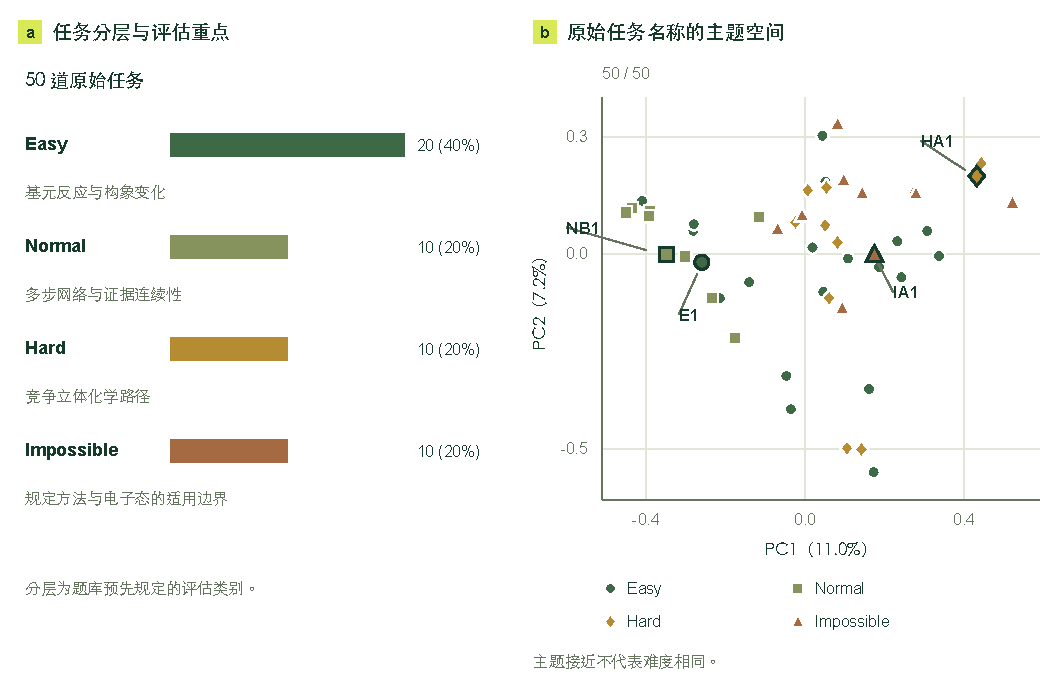
\includegraphics[width=\textwidth]{figures/fig05.pdf}
\caption{CloudraBench 的任务组成与研究主题。a，四档任务的数量及评估重点。b，50 道原始任务名称的 BAAI/bge-m3 嵌入\citep{bgem32024}\ 使用 scikit-learn\citep{sklearn2011}\ 进行主成分分析得到的二维投影，E1、NB1、HA1 和 IA1 为重复实验采用的四题。颜色和点形表示预先规定的任务类别。}
\label{fig:05}
\end{minipage}
\end{figure*}

原子映射系数及 $J_{\min}+2$ 歧义窗口是固定的候选排序启发式。电荷与自由基不匹配的代价高于氢数和键编辑不匹配。支链拥挤度使用衰减 $\rho=0.5$、遍历至深度五和 $B_{\mathrm{axis}}\geq9.0$ 标记。

Cloudra 的构象搜索工具提供 RDKit 和外部 CREST 后端。\citep{crest2020} 可选的 CREST 后端搜索构象或非共价复合物，再进行量子化学优化与物理检验。

\subsection{CloudraBench 基准构建与实验设计}

\subsubsection{任务覆盖与分层依据}

CloudraBench 用 50 题评估端到端机理计算能力：Easy 20 题检验基元转化、构象变化与基础执行可靠性；Normal 10 题检验中间体识别和多步衔接；Hard 10 题检验竞争通道与立体身份；Impossible 10 题检验允许方法下的适用边界与可信否定（图~\ref{fig:05}）。同类反应可因要求研究的路径、构型或电子态不同而分入不同层级。选题依据文献和参考计算，同时考虑能否区分工作流表现及计算成本。配套清单列出各题名称、输入条件和允许方法。



\subsubsection{参考答案与评价方法}

每题固定化学条件、电荷、自旋、交付目标和方法范围。Easy、Normal 和 Hard 任务允许 xTB\citep{gfn2xtb2019}、PM7\citep{pm72013} 与 B3LYP-D3(BJ)/def2-SVP\citep{becke1993,lyp1988,stephens1994,d32010,d3bj2011,def22005}，Impossible 任务限于 xTB 与 PM7；计算证据读取 ORCA、Gaussian 或 MOPAC 原生日志。\citep{orca2025,gaussian16,mopac2026,ref11}\ 参考答案包含物种、基元步、立体身份及适用的数值或否定目标。数值参考按同一方法下的纯电子能差登记，稳定极小值参照与真实 IRC 连接分别核验。对要求验证的可达反应步，我们检查 TS 频率、双向 IRC 及端点优化和频率计算，并核实每个端点优化是否从实际 IRC 末帧出发；物种性质和电子态问题则按其指定目标核验。



图结构、自洽性与准确度分别评价，综合权重为 0.1、0.3 和 0.6；同时报告分级物理支持程度与运行期交付完整性。正确识别方法限制时，按有依据的否定结论计分。



各题列出参考图是否可用、已有参考计算、题目特有的例外处理及尚未完成的验证检查。

\subsubsection{重复实验、主对照与工作流消融}

重复任务研究（P1b）比较 E1、NB1、HA1 与 IA1 在 Guided、Standard、Record 和 Brief-errors 四配置下的表现，每种题目与配置组合独立运行三次，共48次任务运行。重复实验使用 DeepSeek-v4.1-flash（1017）。\citep{deepseekv42026} 四题分别涉及消除预组织、多步脱羧、立体化学开环及电子结构方法边界，其轨迹用于后续局部诊断。耗时单位为并发二、四题一批的实际批次，每配置三批。全基准研究（P2）保留50题、四配置各一次运行，共200次任务运行。全部 P2 配置均通过 DeepSeek 官方端点的流式 OpenAI 兼容 chat completions 接口调用 DeepSeek-v4.1-flash（1017），归档 API 别名为 \texttt{deepseek-v4-flash}，请求 minimal 推理设置。主比较为使用同一主干的 Guided 与 Standard，后者在图中标记为 Backbone。P2 执行版本和请求设置见 SI 第 S1 节。



Standard 隐藏显式 DAG 工具、取消物理检验约束并提供中性计算反馈；Guided 保留研究图、科学检查与详细诊断。Record 保留可用工具和记录，物理检验由运行自行选择；Brief-errors 保留引导而缩短诊断。各配置采用相同题目与方法限制；档案保存各次运行的代码版本、预算、结束原因及其计算源文件。



评分前，人工依据各次运行的对话、工具记录、报告和计算文件，按 Agent 表达的机理意图与结论重建机理图，恢复文件引用，并记录每个恢复字段的来源。重建仅使用该次运行已有的计算和结论。评分器在其沙箱中搜索原生计算证据，按统一规则对照 Gold 目标评分。最终数据包含全部200次运行，每项综合分均列出对应的图结构、自洽性和准确度。逐题配对差及95\%百分位区间采用100,000次任务簇 bootstrap，同一任务的四配置始终一起抽样，随机种子为20261031。计算投入取四配置均有记录的15道选定任务，报告量子化学作业数和累计 job-hours。

